\acrshort{surf} showed vastly different results then expected.
The first observation is that the sheer numbers of detected keypoints with default settings are rendering the keypoint classification results meaningless.
After some experimentation with the settings it became clear, that on each octave and every blurring convolution a high number of keypoints are detected redundantly.
This finding was true for both the \glspl{flexion-image} and \glspl{bearing-angle-image}, resulting in a suboptimal keypoint detector performance in scale space.
In theory, different keypoint detectors can be combined with different keypoint descriptors and as \acrshort{surf} is commonly referred to as the faster \acrshort{sift}, its description potential should still be evaluated.
The default settings for \acrshort{surf} are still used, but only one octave with four blurring convolutions detects keypoints (Figure~\ref{fig:surf_keypoints_mess}), resulting in the keypoint statistics presented in Table~\ref{tab:surf_results}.
% \vspace{-2mm}
\begin{figure}[t]
\begin{subfigure}[t]{0.25\linewidth}
    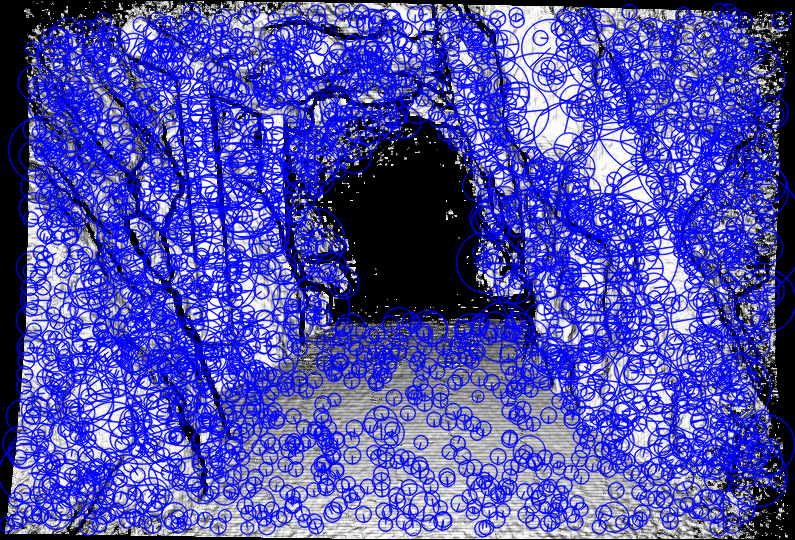
\includegraphics[width=\linewidth]{chapter06/results/SURF/flexion/default_kp0005.png}%
\end{subfigure}%
\begin{subfigure}[t]{0.25\linewidth}
    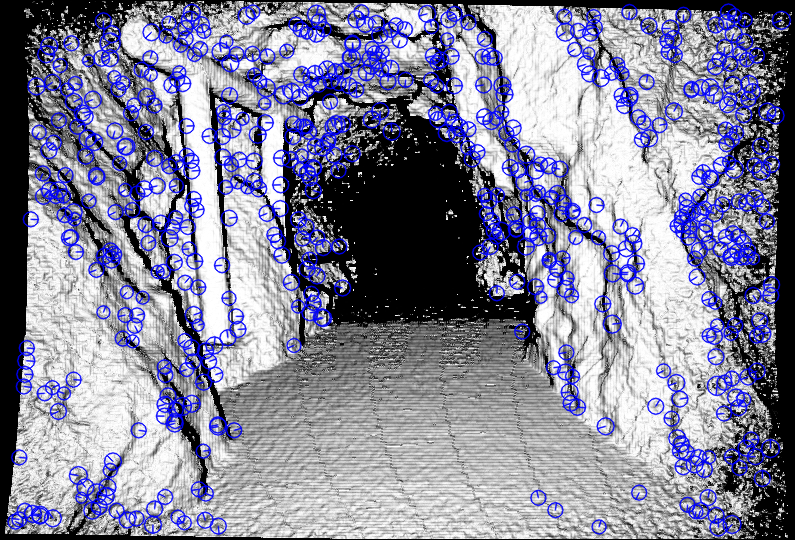
\includegraphics[width=\linewidth]{chapter06/results/SURF/flexion/oneoctave_kp0005.png}%
\end{subfigure}%
\begin{subfigure}[t]{0.25\linewidth}
    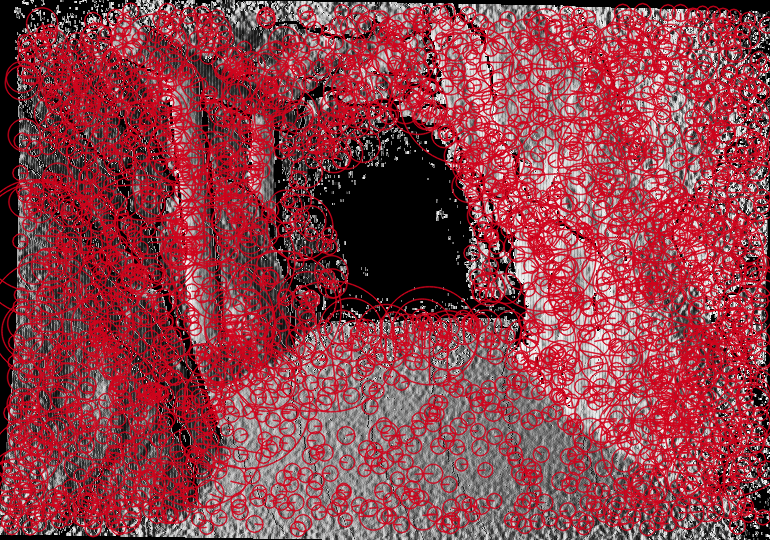
\includegraphics[width=\linewidth]{chapter06/results/SURF/bearing/default_kp0005.png}%
\end{subfigure}%
\begin{subfigure}[t]{0.25\linewidth}
    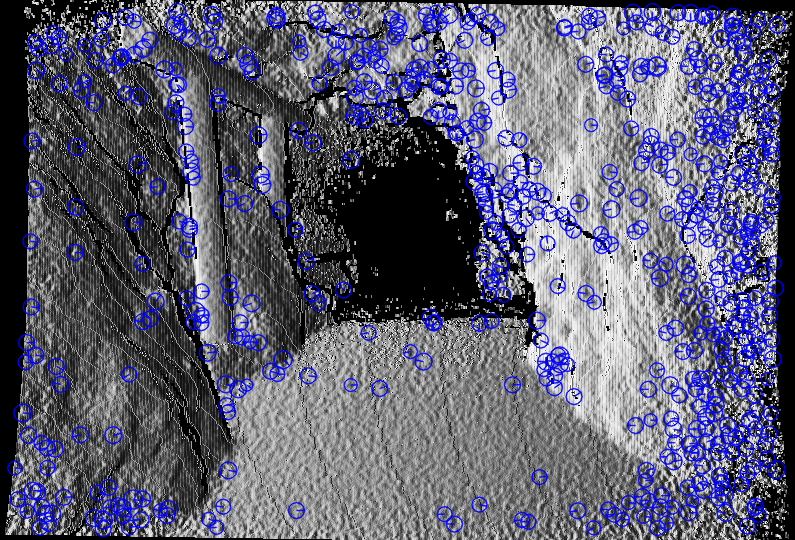
\includegraphics[width=\linewidth]{chapter06/results/SURF/bearing/oneoctave_kp0005.png}%
\end{subfigure}%
    \caption[\acrshort{surf} keypoints plotted in feature images]{\emph{\acrshort{surf} keypoints plotted in feature images.} This figure shows the number of keypoints that are detected with \acrshort{surf} in its default configuration compared to just using one octave. Limiting the number of keypoints is mandatory to achieve some potentially meaningful result.}\label{fig:surf_keypoints_mess}
\end{figure}
% \vspace{-8mm}
\begin{table}[b!]
    {\renewcommand{\arraystretch}{1.2}%
    \setlength{\tabcolsep}{0.7em}%
    \footnotesize
\begin{tabular}{bababab}
\toprule

\rowcolor{white} \null &
\textbf{Synthetic$_{\mathbf{\mathcal{F}}}$} & \textbf{Synthetic$_{\mathbf{\mathcal{\beta}}}$} &
\textbf{Mine$_{\mathbf{\mathcal{F}}}$} & \textbf{Mine$_{\mathbf{\mathcal{\beta}}}$} &
\textbf{Office$_{\mathbf{\mathcal{F}}}$} & \textbf{Office$_{\mathbf{\mathcal{\beta}}}$} \\
\midrule

\rowcolor{lightgray}
\textbf{Keypoint Count} &
    \num{105788} & \num{23203} &
    \num{440400} & \num{440400} &
    \num{34200} & \num{34200} \\
\textbf{Correspondences} &
    \num{28836} & \num{5221} &
    \num{23132} & \num{13846} &
    \num{4172} & \num{2859} \\
\rowcolor{lightgray}
\textbf{True Positives} &
    \num{14047} & \num{3186} &
    \num{7688} & \num{2003} &
    \num{2131} & \num{1223} \\
\textbf{False Positives} &
    \num{27884} & \num{6148} &
    \num{144506} & \num{137922} &
    \num{10734} & \num{10632} \\
\rowcolor{lightgray}
\textbf{False Negatives} &
    \num{14789} & \num{2035} &
    \num{15444} & \num{11843} &
    \num{2041} & \num{1636} \\
\textbf{Precision} &
    \num{0.335} & \num{0.341} &
    \num{0.051} & \num{0.014} &
    \num{0.166} & \num{0.103} \\
\rowcolor{lightgray}
\textbf{Recall} &
    \num{0.487} & \num{0.610} &
    \num{0.332} & \num{0.145} &
    \num{0.511} & \num{0.428} \\
\textbf{Youden's index} &
    \num{0.123} & \num{0.268} &
    \num{-0.015} & \num{-0.179} &
    \num{0.146} & \num{0.082} \\
\rowcolor{lightgray}
\textbf{Accuracy} &
    \num{0.595} & \num{0.647} &
    \num{0.636} & \num{0.660} &
    \num{0.620} & \num{0.635} \\
\bottomrule
\end{tabular}

    }
    \caption[Keypoint and matching result for \texttt{\acrshort{surf}/raw/best-only}]{\emph{Keypoint and matching result for \texttt{\acrshort{surf}/raw/best-only}.} The Youden index around 0.1 and even below 0 already indicates bad performance. The number of keypoints is still substantially higher than for \acrshort{sift}, even with the limit of the keypoint count and usage of only one octave.}\label{tab:surf_results}
\end{table}
The number of correspondences for the adjusted \acrshort{surf} setup is comparable to \acrshort{sift} detecting keypoints on multiple scales.
But the high number of false negatives already indicates lesser descriptor performance.
This impression is solidified with the descriptor distance analysis in Figure~\ref{fig:surf_descriptor_distance}.
\begin{figure}[htb]
\begin{subfigure}[t]{0.45\linewidth}
    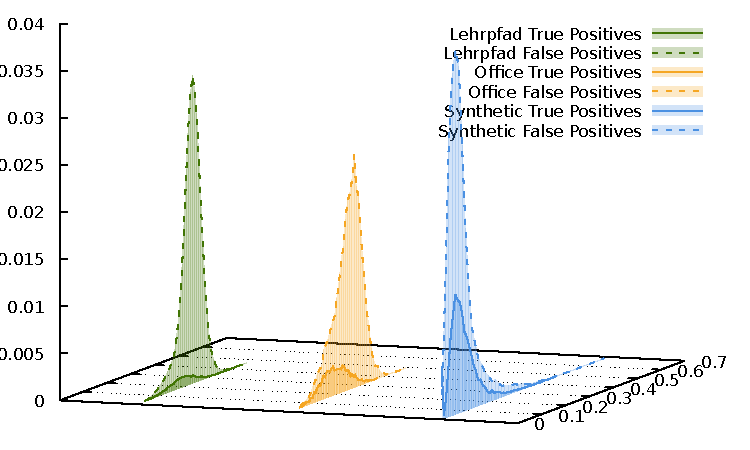
\includegraphics[width=\linewidth]{chapter06/results/SURF/flexion/descriptor_distances.pdf}%
    \caption{\gls{flexion-image}}
\end{subfigure}\quad
\begin{subfigure}[t]{0.45\linewidth}
    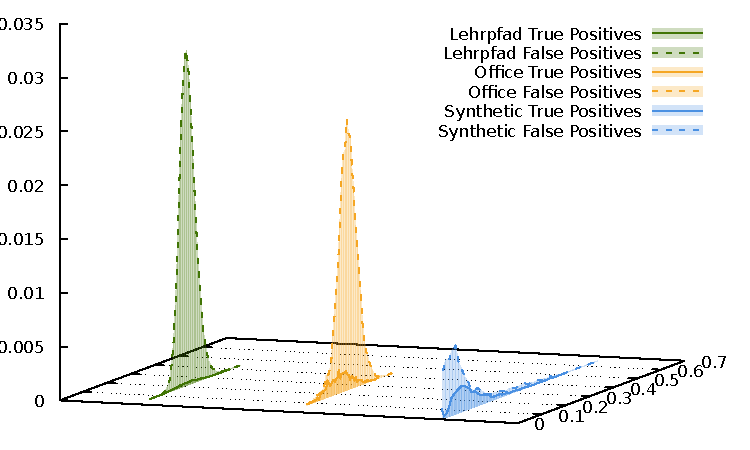
\includegraphics[width=\linewidth]{chapter06/results/SURF/bearing/descriptor_distances.pdf}%
    \caption{\gls{bearing-angle-image}}
\end{subfigure}
\caption[\acrshort{surf} descriptor distances]{\emph{\acrshort{surf} descriptor distances.} The descriptor of \acrshort{surf} does not discriminate regions well. True positives barely separate from false positives.}\label{fig:surf_descriptor_distance}
\end{figure}
A slight separation of true and false positives exists for \glspl{flexion-image}, which is not the case for \glspl{bearing-angle-image}.
Even this slight separation is neglected by drastically higher numbers of false positives.
Separating both distributions through a maximum matching distance is hard to justify.
For a 64 element descriptor that \acrshort{surf} deploys, the match distance around \num{0.3} seems very low, too.
The \acrshort{ROC} analysis (Figure~\ref{fig:roc_surf}) points in the same direction showing performance around the \emph{Random Guess} quality, for \emph{Mine} even below.
\begin{figure}[b!]
\begin{subfigure}[t]{0.45\linewidth}
    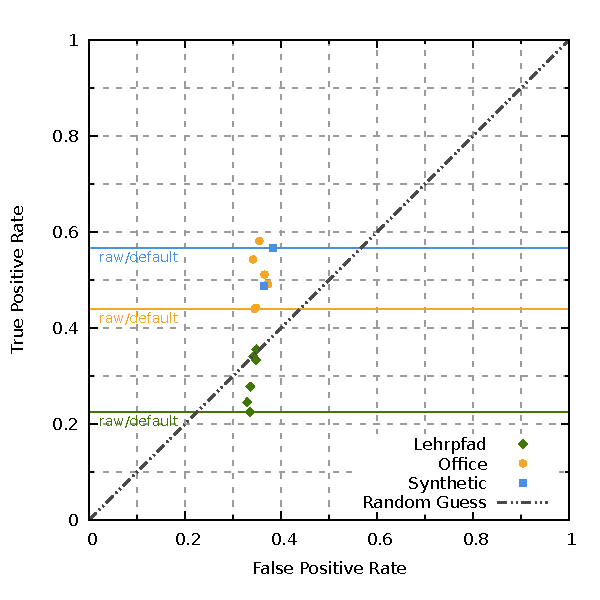
\includegraphics[width=\linewidth]{chapter06/results/SURF/flexion/roc.pdf}%
    \caption{\gls{flexion-image}}
\end{subfigure}\quad
\begin{subfigure}[t]{0.45\linewidth}
    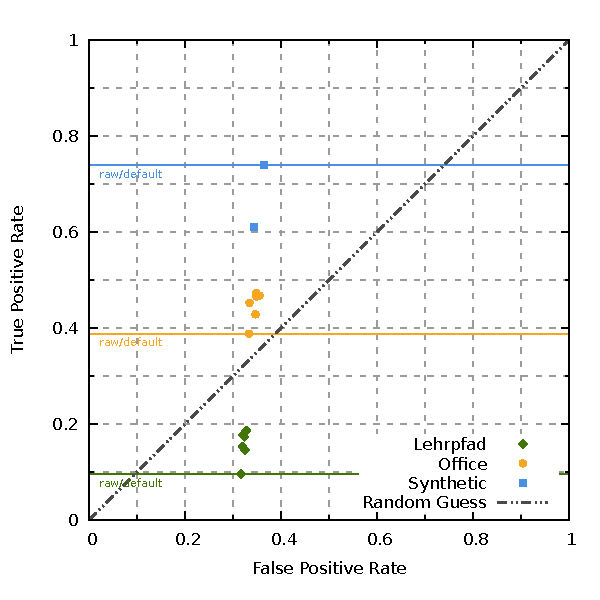
\includegraphics[width=\linewidth]{chapter06/results/SURF/bearing/roc.pdf}
    \caption{\gls{bearing-angle-image}}
\end{subfigure}
\caption[The \acrshort{ROC} graphs for \acrshort{surf}]{\emph{The \acrshort{ROC} graphs for \acrshort{surf}.} No metric for \acrshort{surf} shows any indication of a good classification for correspondences. The \acrshort{ROC} graph underlines, that no configurations or data preprocessing substantially improves the situation.}\label{fig:roc_surf}
\end{figure}
The suspected reason for this poor performance of \acrshort{surf} is the use of the Haar-Wavelet response as key metric of the descriptor.
The feature image conversions do not result in sharp edges of brightness, as is the case for classical color images and the textures on real world objects.
As the feature images result in more subtle gray changes, \acrshort{surf} looses its descriptive power.
This evaluation needs to be taken into account when comparing to prior results of Lin et al.\cite{lin_easp2017}.
The registration performance use the \glspl{bearing-angle-image} was inferior to a classical \acrshort{icp} but improved its convergence speed.
\acrshort{surf} can produce true keypoint correspondences for some datasets and with the use \acrshort{RANSAC} an approximate pose estimation is thinkable.
Nonetheless, \acrshort{surf} falls flat compared to \acrshort{sift} and should not be used on the proposed feature images.
Appendix~\ref{sec:surf_stats} presents additional statistics for the \acrshort{surf} keypoints.
